\documentclass[../../main.tex]{subfiles}

\begin{document}
    
    Nach Einbau des Resonatormoduls G 

    \begin{figure}
        \centering
        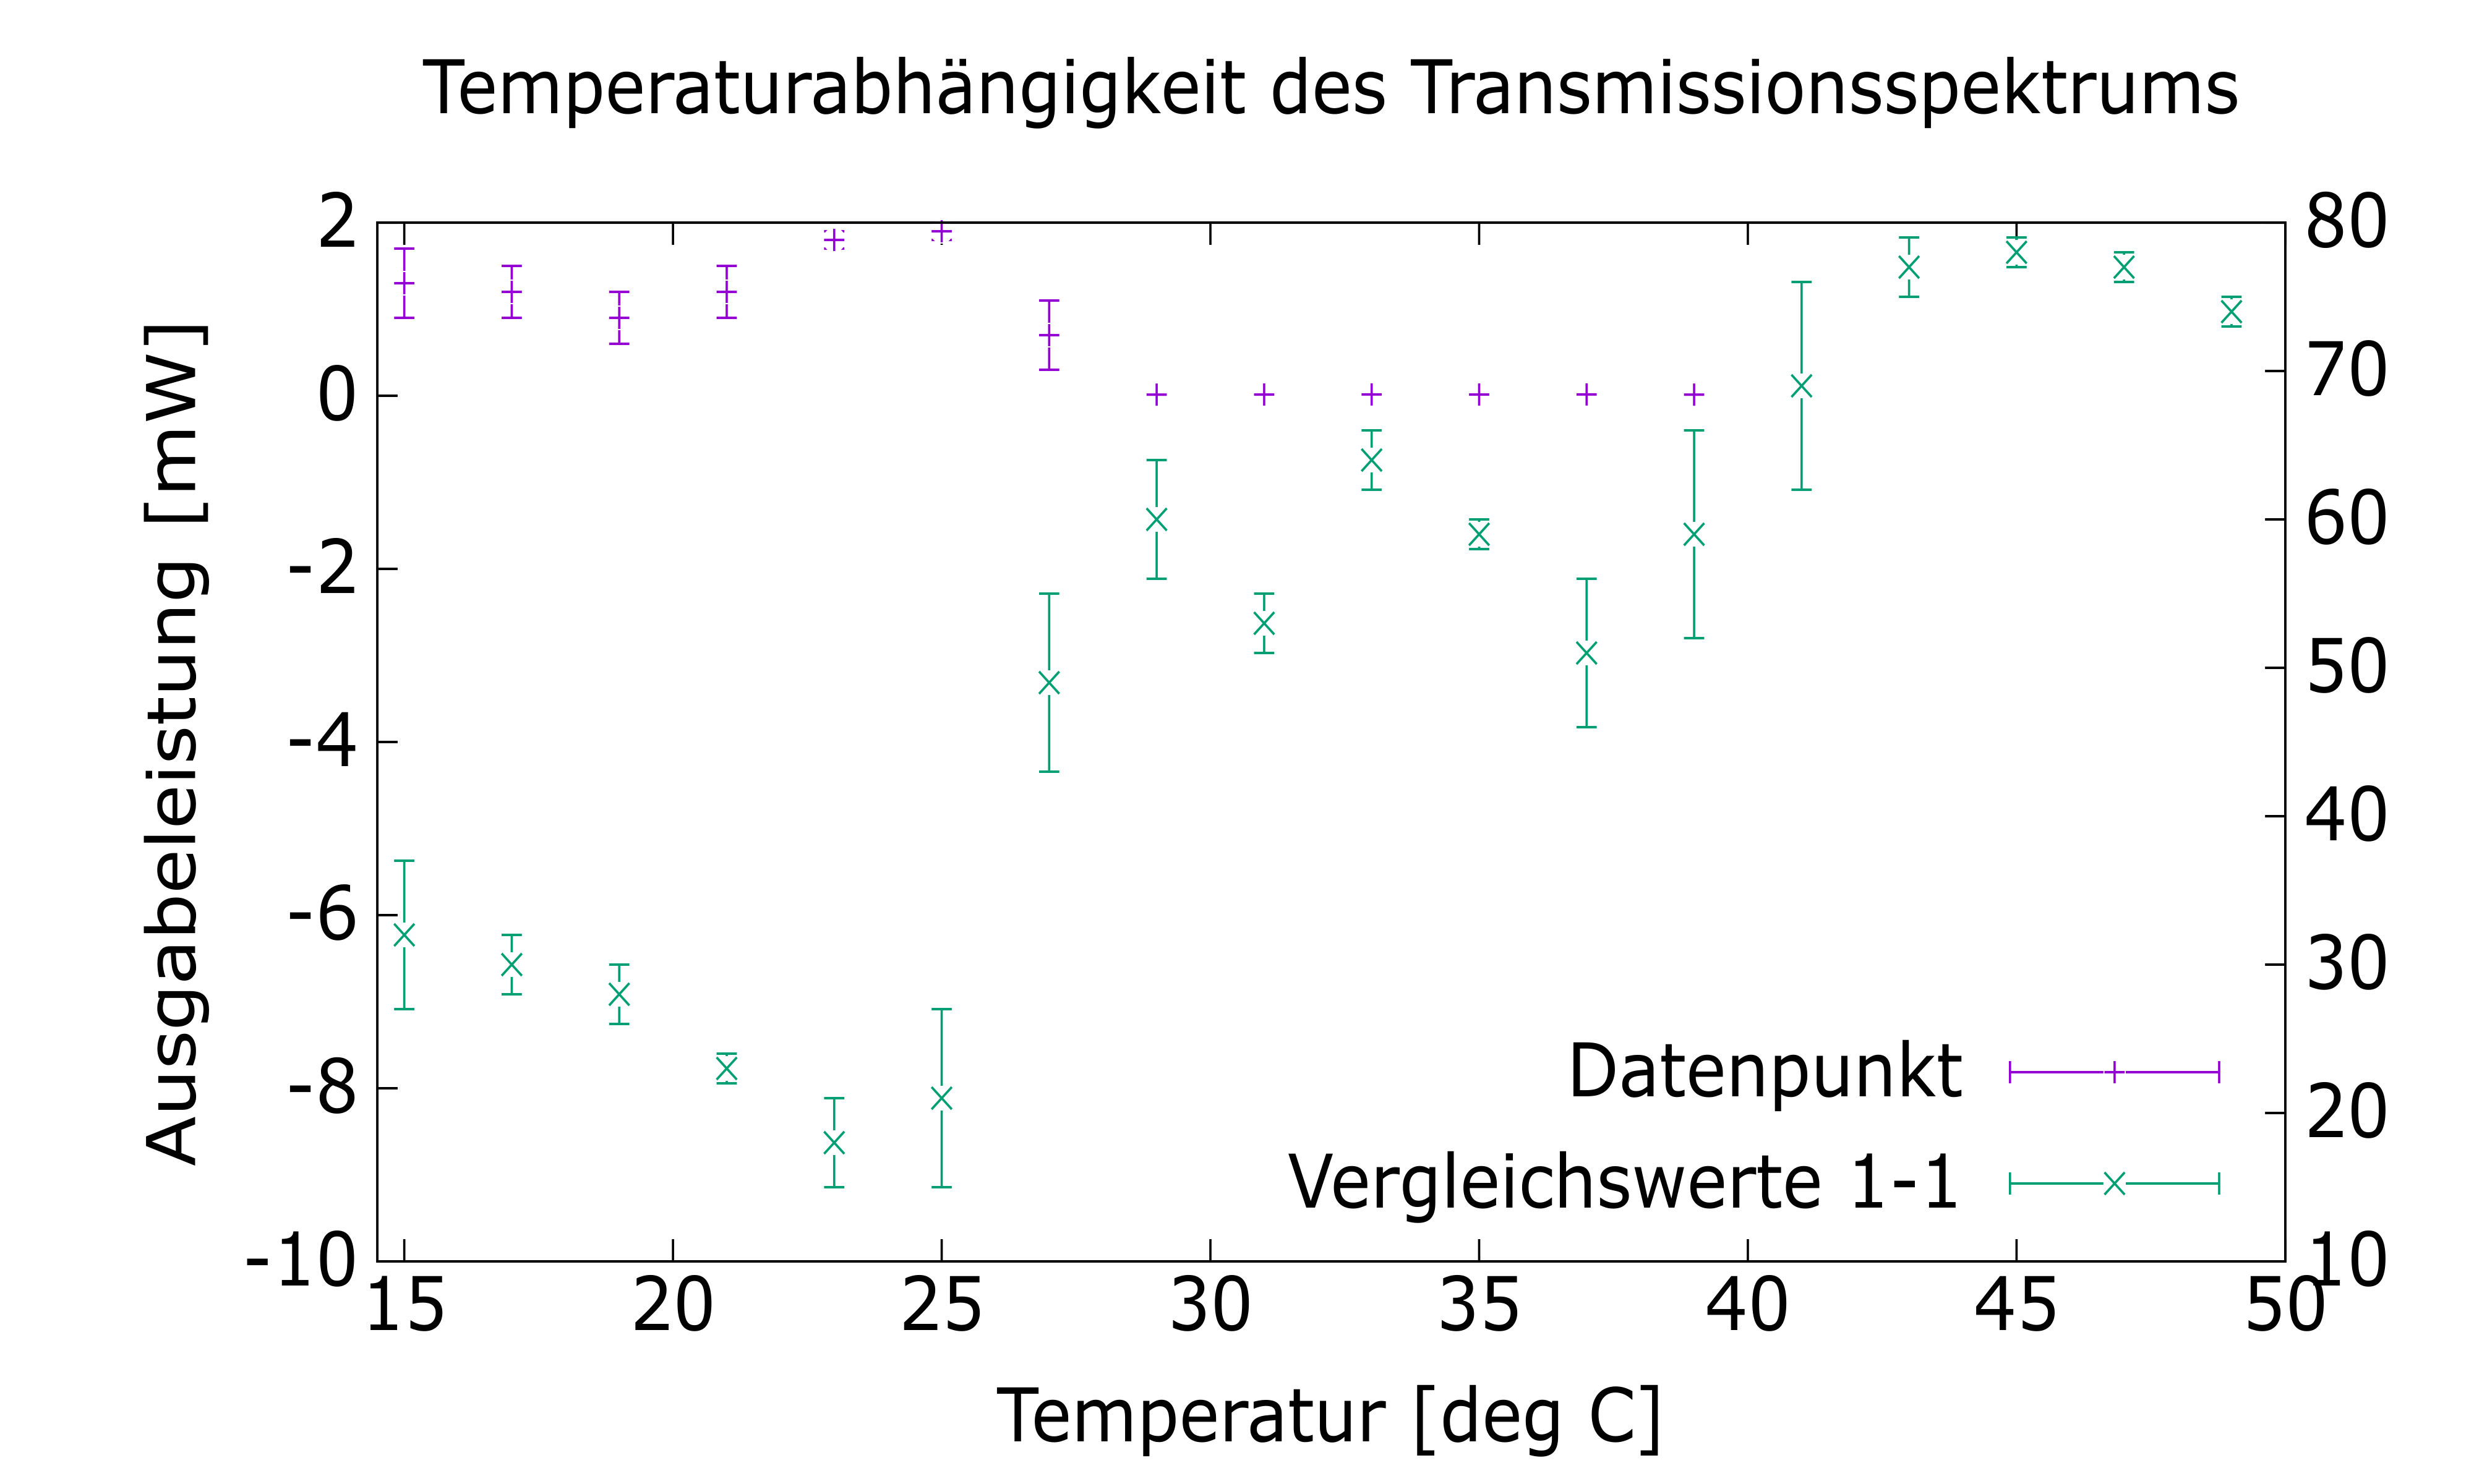
\includegraphics[width=11cm]{../../Bilddateien/4/PowerOverTemperature_400mA_comp.png}
        \caption{Die Ausgangsleistung des Nd:YAG Lasers als Funktion der Temperatur bei konstantem Anregungsstrom $I_{\textit{an}} = 400\si{\mA}$, verglichen mit dem Transmissionsspektrum des Nd:YAG Kristalls aus Kapitel \ref{subsec:1-1:Diodenlasertemperaturoptimierung}.}
    \end{figure}

    \begin{figure}
        \centering
        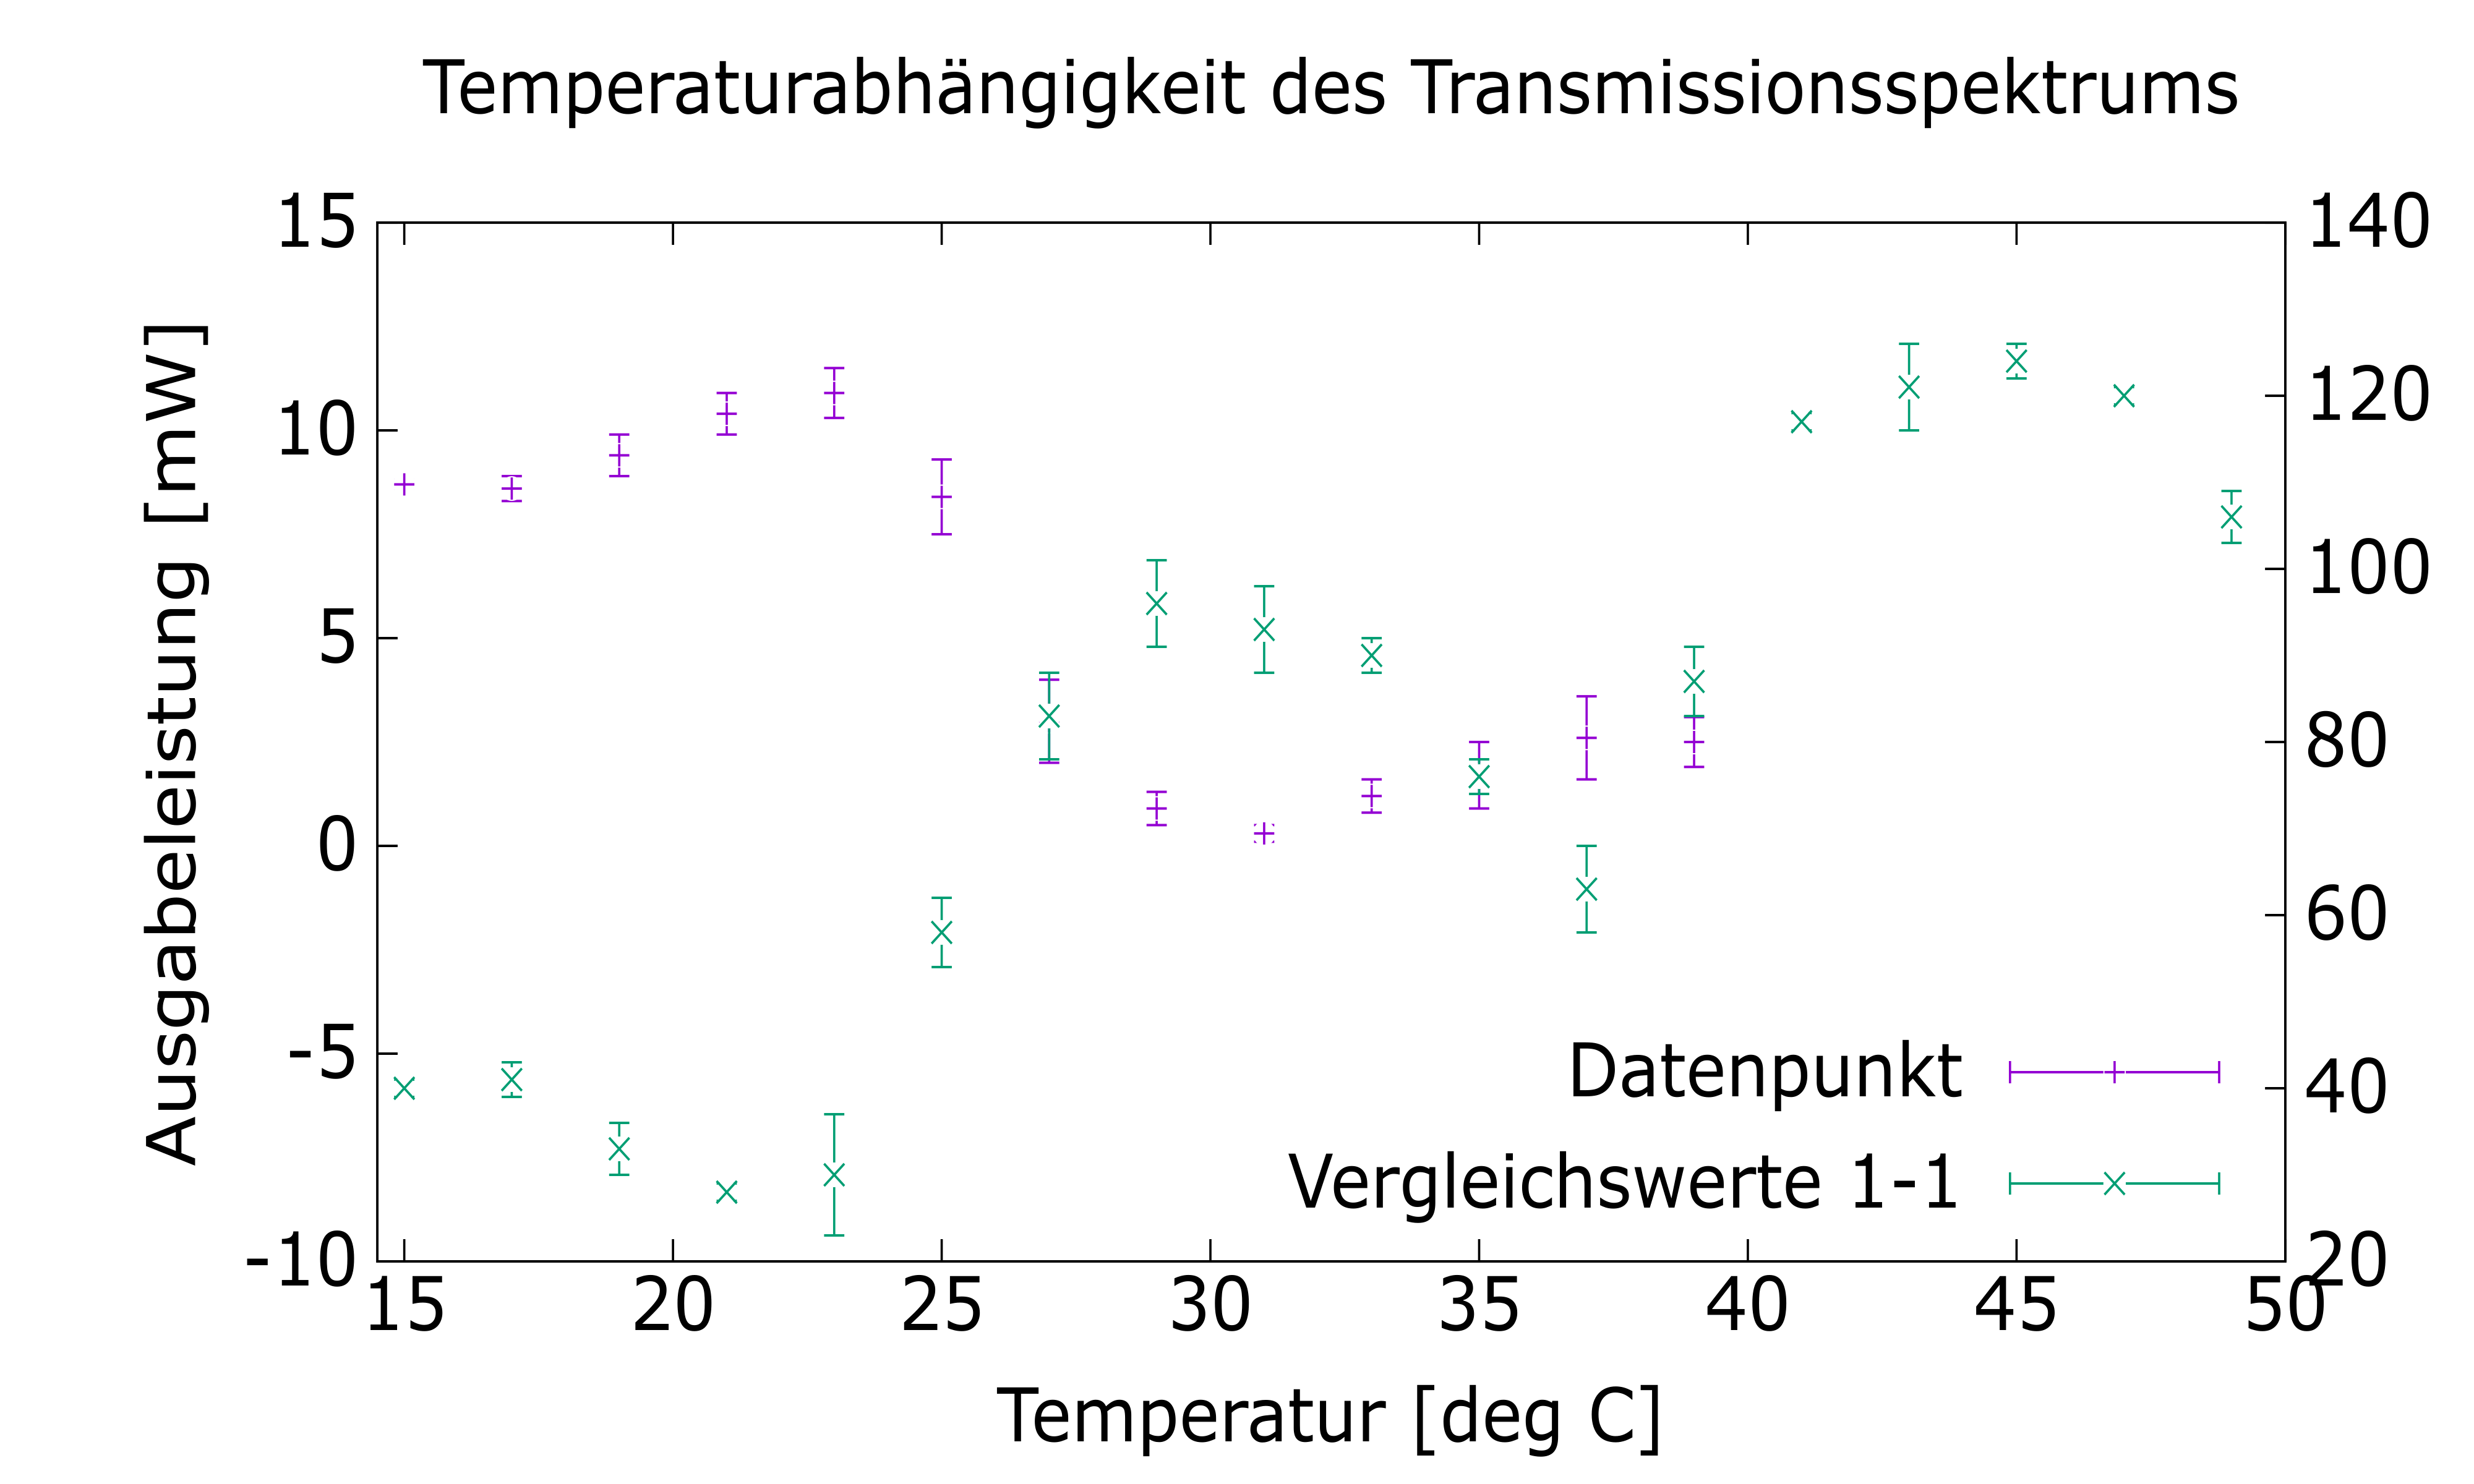
\includegraphics[width=11cm]{../../Bilddateien/4/PowerOverTemperature_550mA_comp.png}
        \caption{Die Ausgangsleistung des Nd:YAG Lasers als Funktion der Temperatur bei konstantem Anregungsstrom $I_{\textit{an}} = 550\si{\mA}$, verglichen mit dem Transmissionsspektrum des Nd:YAG Kristalls aus Kapitel \ref{subsec:1-1:Diodenlasertemperaturoptimierung}.}
    \end{figure}

\end{document}